\chapter{Pilots}
We conducted two pilots, the first one did not include the implementation of questions of varying difficulty and the second one did. The main objective when implementing this new question generating algorithm was to try and bring the players closer to a 50\% success rate when answering questions
\section{First pilot}\label{sec:pilot1}
We made Reminisce.me available to the public and asked family and friends to play the game. Over the course of roughly one week people have answered 1227 over the course of 83 games. We had 25 users which brings us to an average of 3.32 games played by user.
\subsection{Selected Questions}
During this trial, people answered 377 order questions, 348 timeline questions, 317 multiple choice questions and 185 geolocation questions. Of those questions 159 order questions, 174 timeline questions, 192 multiple choice questions and 158 geolocation questions were correct.\\
An other interesting statistics is the number of avoided questions. Without taking into account the state of the board, one can see that 407 order questions, 502 timeline questions, 443 multiple choice questions and 142 geolocation questions were not answered. Aside from random factors (such as the position of the board, which questions were locked etc...), this statistics can be explained by two main factors: the fun of playing a certain question type and the perceived difficulty. While there is nothing that can be said about order question (the number of answered ones is close to the number of avoided ones), it seems like people have a tendency to avoid timeline and multiple choice questions and based on the feedback we got from the users, it might be linked to the perceived difficulty. On the other hand the geolocation are picked with a visibly high ratio. The high success rate on this kind of question is probably a good explanation. Figure \ref{fig:p1TotCorrectAvoid} shows a summary of those results.
\begin{figure}
\centering
{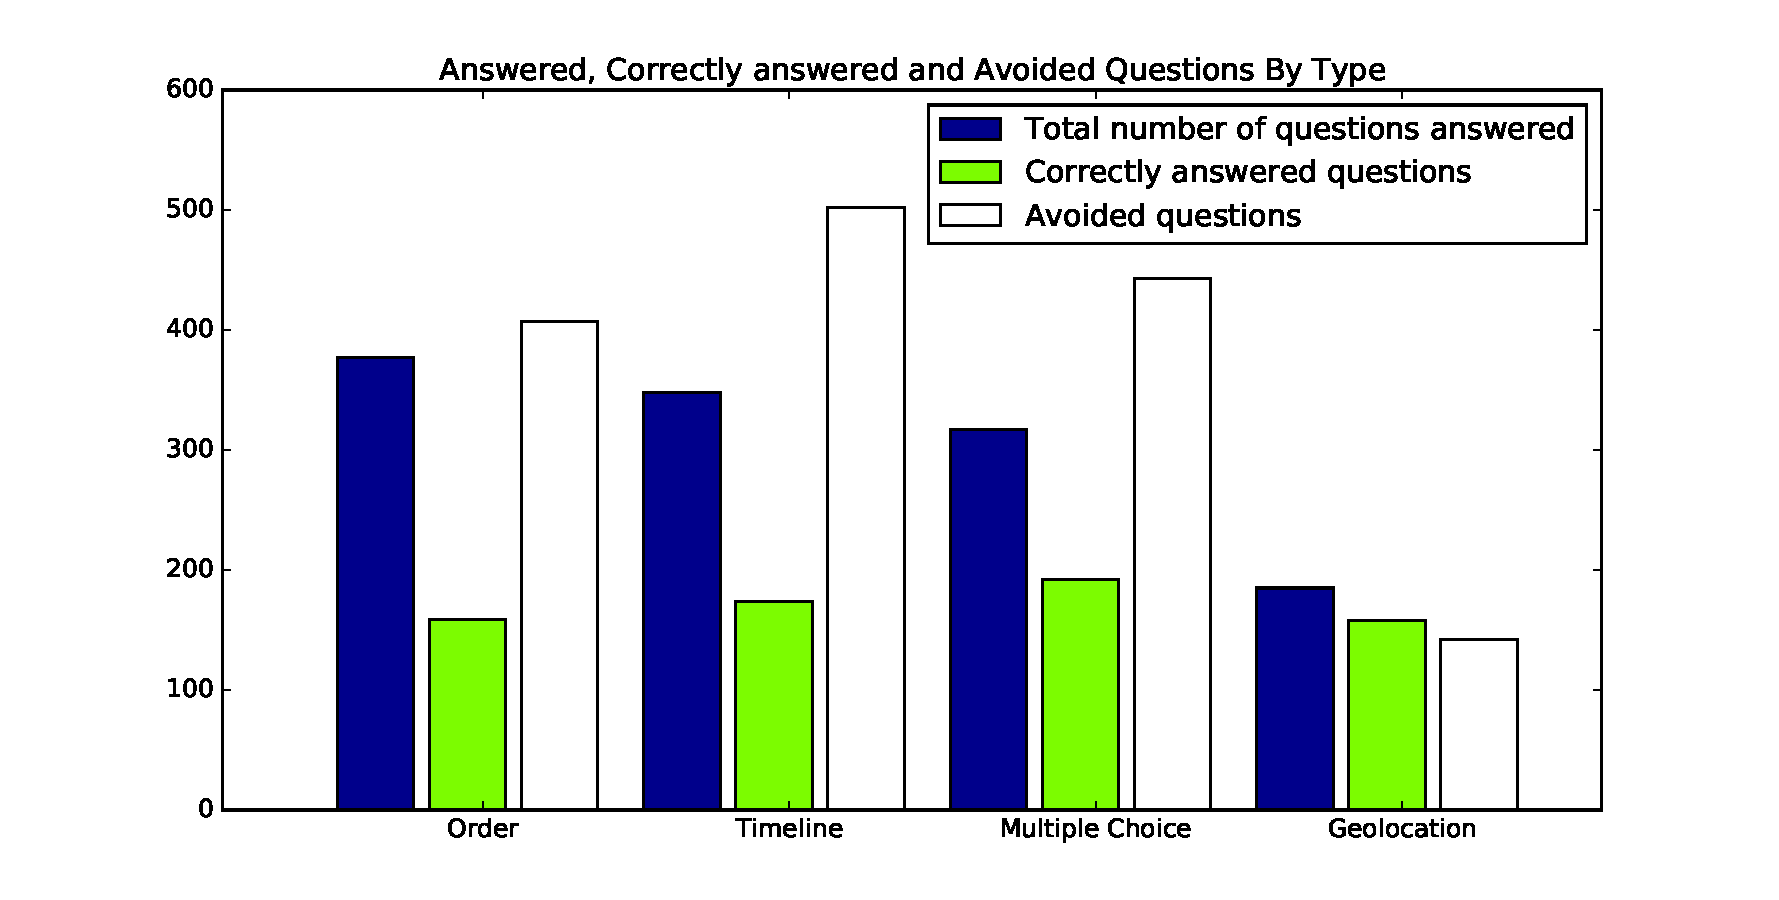
\includegraphics[width=4in]{images/pilot_1_selected_questions.pdf}}
\caption{Total, Correct and Avoided Questions Answered By Type}
\label{fig:p1TotCorrectAvoid}
\end{figure}
\subsection{Remembered Or Randomly Selected}
As for the pilot in June 2016, we can conclude that on average the players tend to try and remember the answers. The average performance for ordering questions was 35.04\% success rate while when answering at random would yield a 16.67\% success. For timeline we get a 51.07\% success which is more than the 33.33\% random success rate. The result is the same for the multiple choice questions with respectively 58.6\% and 25\% for the measured and random success rate. Finally we measured an extraordinary 61.5\% average success rate on the geolocation. While this last result is impressive it came with a rather high standard deviation and, given the low number of localized posts, the amount of different questions is low and most of the players would be able to learn the answers by heart. Figure \ref{fig:p1Correct} shows a summary of those results.\\
The high variance makes it hard to see how most of the users behaved. The box plot shown on figure \ref{fig:p1Boxes} tells us that for the timeline questions, more than 75\% of users were better than random and that half of the user had between 40\% and 60\% success, which approximately what we wish to achieve with the difficulty in the second pilot. For order questions, more than half of the participants were better than random but most of the users had a success rate between 15\% and 51\% which is way too low so we would expect the difficulty to improve those results. The multiple choice results give that more than 75\% of the players were better than the random choice and for most of the people the average success rate was between 45\% and 75\%. This is a bit too high and we would expect that the implementation of difficulty would reduce that. When it comes to the geolocation questions we run into some issues, most of the people who had some of them had a success rate between 90\% and 100\%, this corroborates the hypothesis that most of the people who have this kind of question have so few that they can memorize them.
\begin{figure}
\centering
{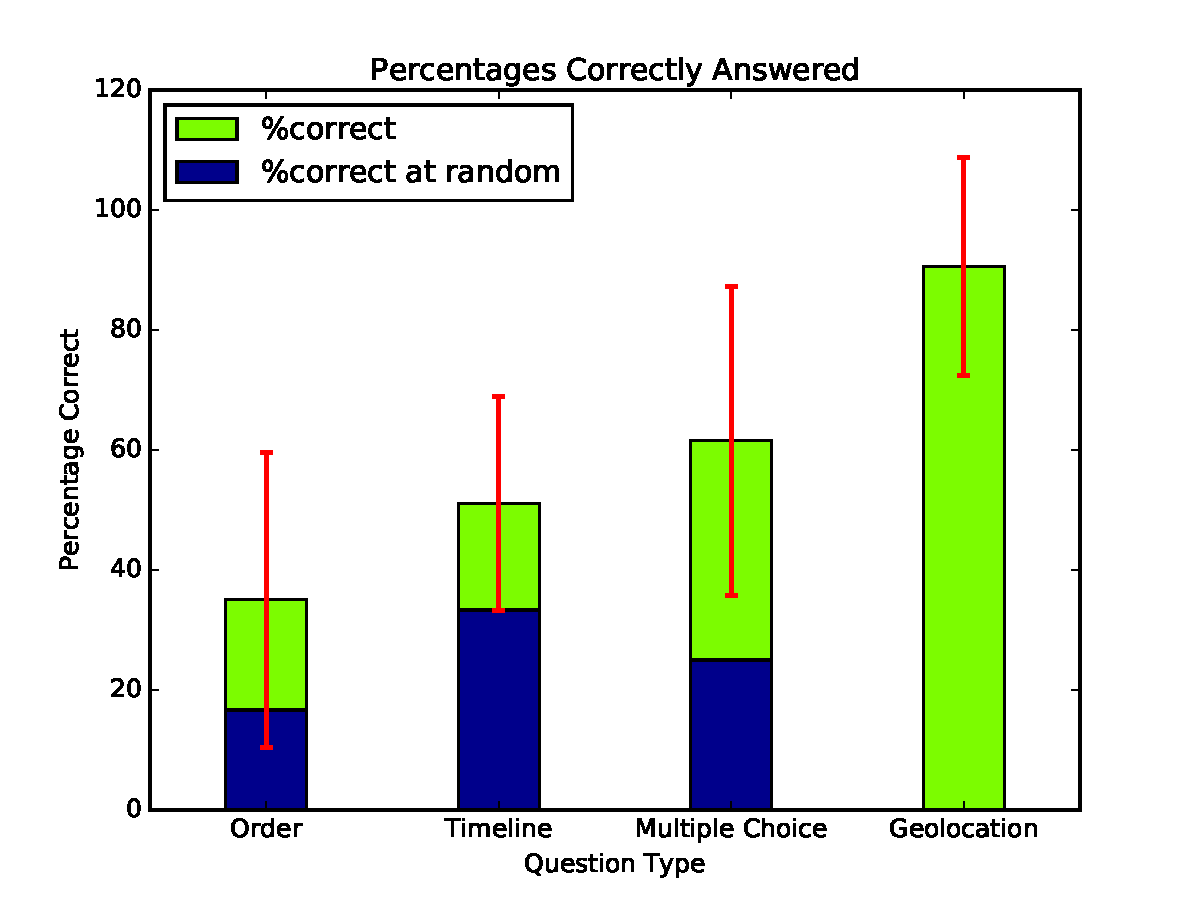
\includegraphics[width=4in]{images/pilot_1_correct.pdf}}
\caption{Percentages Correctly Answered}
\label{fig:p1Correct}
\end{figure}
\begin{figure}
\centering
{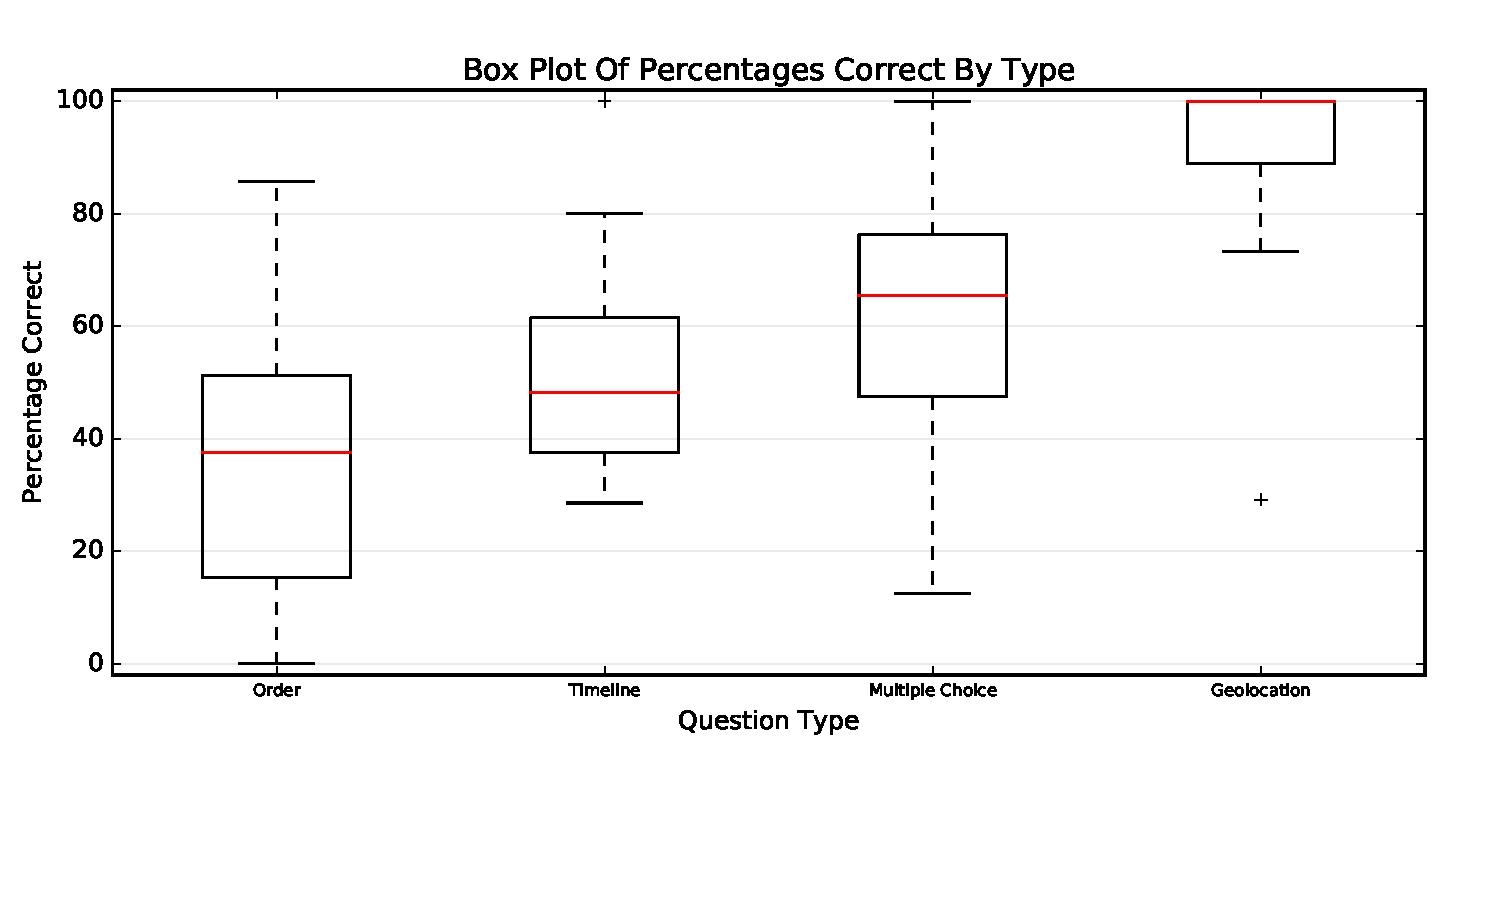
\includegraphics[width=4in]{images/pilot_1_boxplot.pdf}}
\caption{Percentages Correctly Answered Box Plots}
\label{fig:p1Boxes}
\end{figure}

\section{Time spent}
Figure \ref{fig:p1BoxesTime} shows that the time spent on timeline and multiple choice questions is pretty similar, it is a little higher for the multiple choice questions which can be explained by the higher number of possible answers. The ordering questions take more time probably because of the time taken for dragging the items. The most time is spent on the geolocation questions, it seems that there is some more thinking and the players might also be slowed down by the time taken to type their answer. However, it does not indicate that remembering a place is harder as the success rate on this kind of question is really high.
\begin{figure}
\centering
{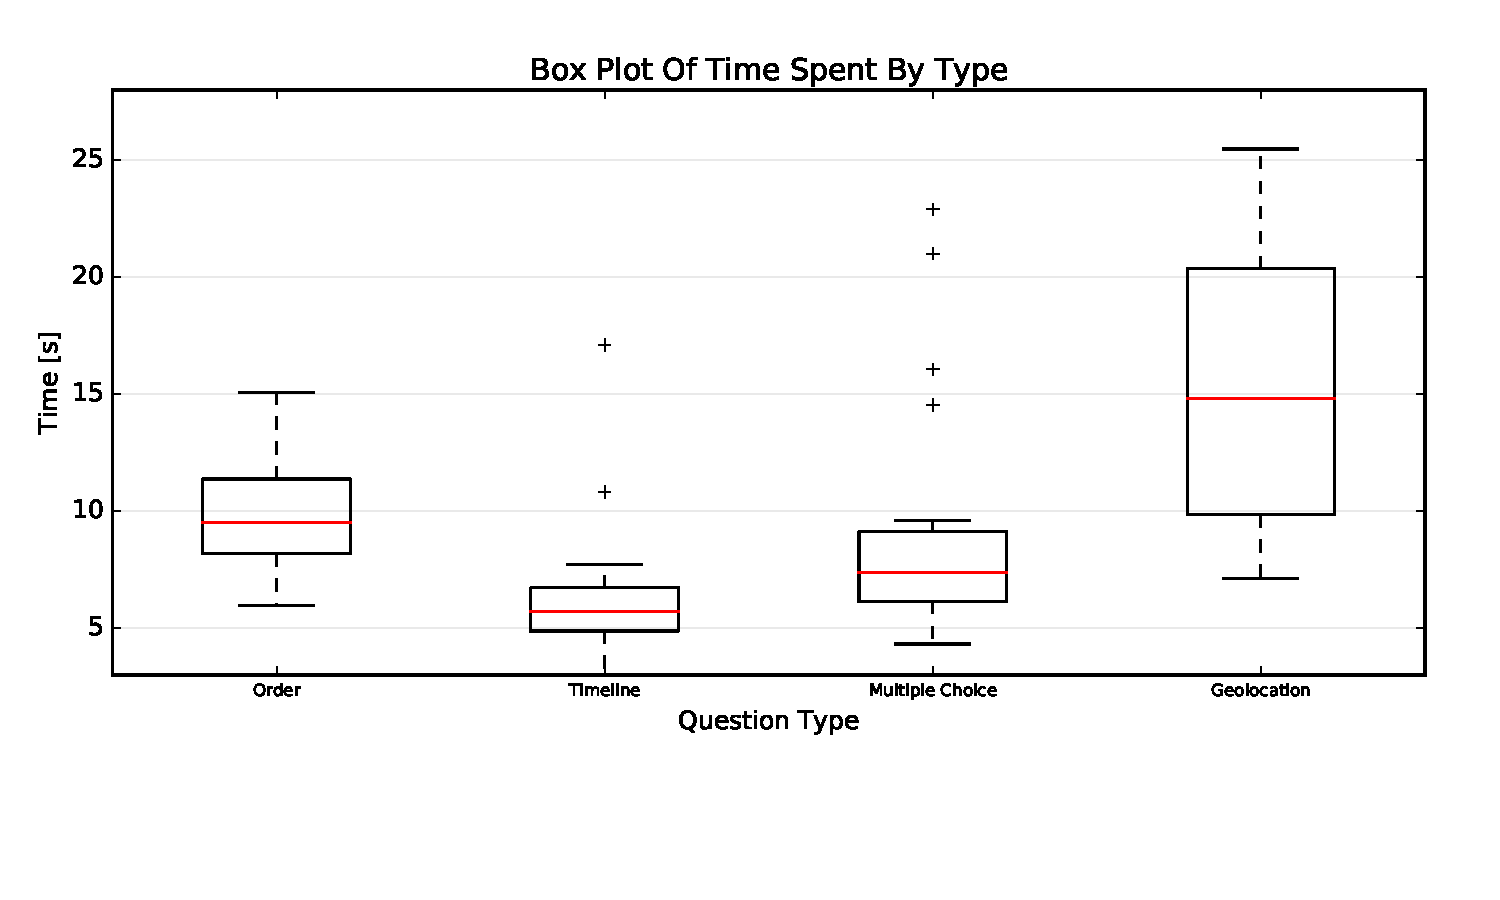
\includegraphics[width=4in]{images/pilot_1_boxplot_time.pdf}}
\caption{Box Plots Of Time Spent By Type}
\label{fig:p1BoxesTime}
\end{figure}

\section{Second pilot: on the influence of difficulty}
Following the same procedure, we asked friends and family to play the game. Over a bit more than a week, 40 different users played 155 games (on average 3.88 games per person) and answered 2517 questions. For this second pilot, we will perform the same general analysis and then dive in individual question types to try and see the impact of the difficulty.

\subsection{Selected Questions}
During this trial, people answered 546 order questions, 1022 timeline questions, 688 multiple choice questions and 261 geolocation questions. Of those questions 289 order questions, 592 timeline questions, 457 multiple choice questions and 223 geolocation questions were correct.\\
As for avoiding questions, 583 order questions, 1703 timeline questions, 815 multiple choice questions and 352 geolocation questions were avoided. This time we see an even clearer avoidance of timeline questions, a bit less avoidance than before for multiple choice questions and the geolocation questions are no longer picked as much. It is hard to interpret these results as the avoidance count does not take into account the board state at all which can have a huge influence on the result. It would be better to improve this measurement before trying to deduct anything. Figure \ref{fig:p2TotCorrectAvoid} shows a summary of those results.
\begin{figure}
\centering
{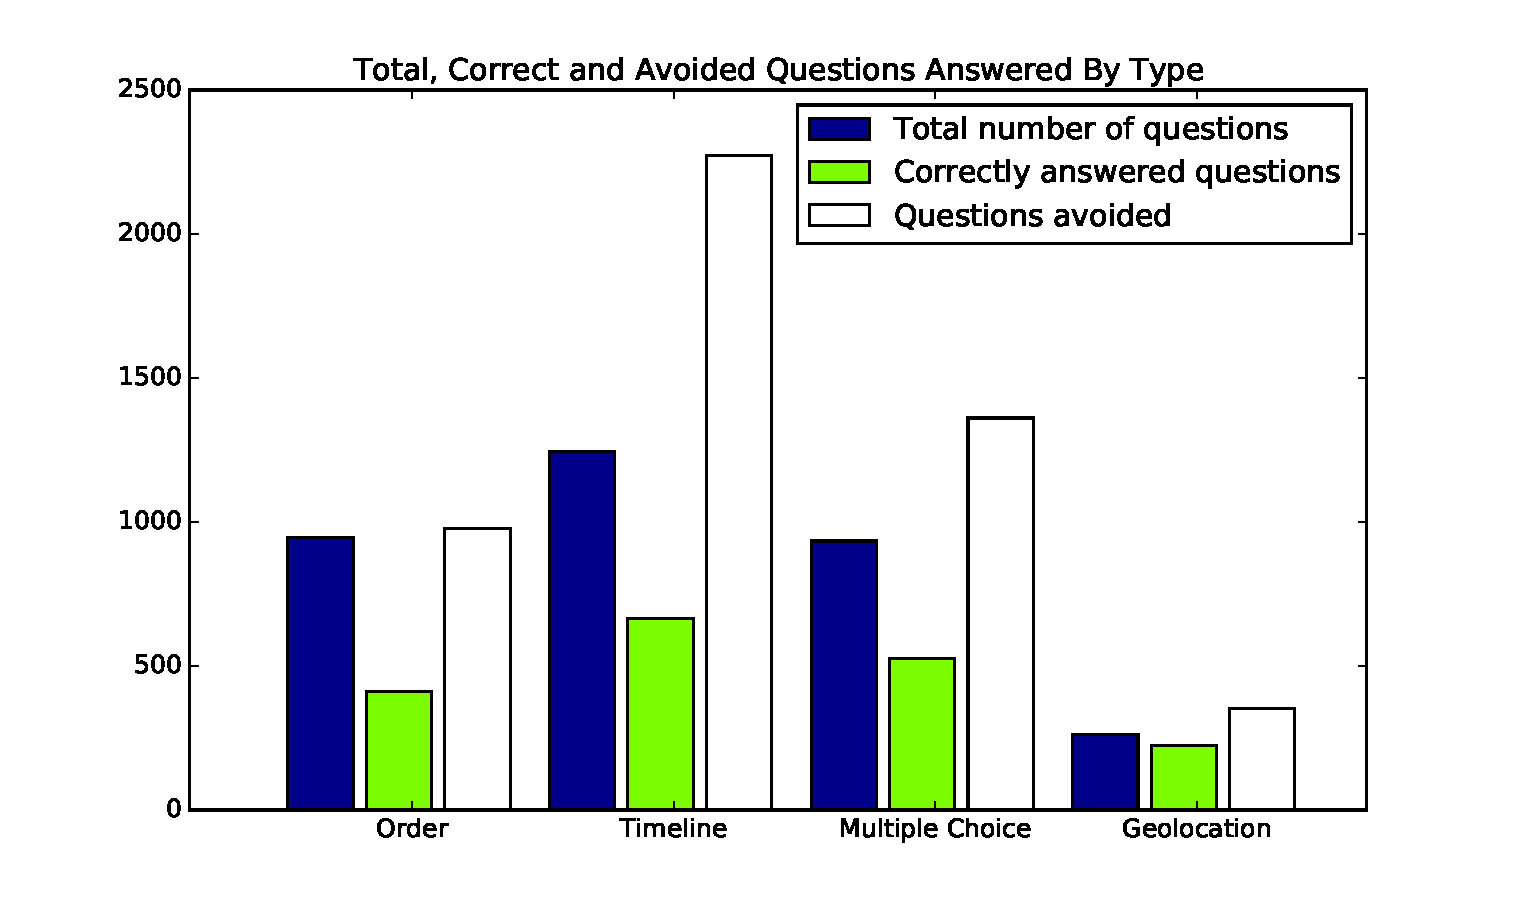
\includegraphics[width=4in]{images/pilot_2_selected_questions.pdf}}
\caption{Total, Correct and Avoided Questions Answered By Type}
\label{fig:p2TotCorrectAvoid}
\end{figure}
\subsection{Remembered Or Randomly Selected}\label{sec:p2remem}
On this pilot again we can again conclude that on average the people did not select their answer at random. The order questions were answered on average 48.63\% of the time correct, the timeline questions were answered correctly 56.78\% of the time and the multiple choice questions were answered correctly 66.69\% of the time. The really impressive result comes from geolocation questions, they were answered correctly a staggering 92.3\% of the time with a rather low standard deviation. Some more analysis on this particular result is done on section \ref{subsec:explained}. Figure \ref{fig:p2Correct} shows an overview of these numbers.\\
As before a box plot (figure \ref{fig:p2Boxes}) can help us understand the data better. We see that this time, most of the people had between 42\% and 52\% success on the ordering questions. For timeline questions, most of the participant found themselves between 40\% and 67\% correct answers. When it comes to multiple choice questions, most of the participants find themselves between 50\% and 84\%. Finally, geolocation answers where mostly comprised between 87\% and 100\% correct.

\begin{figure}
\centering
{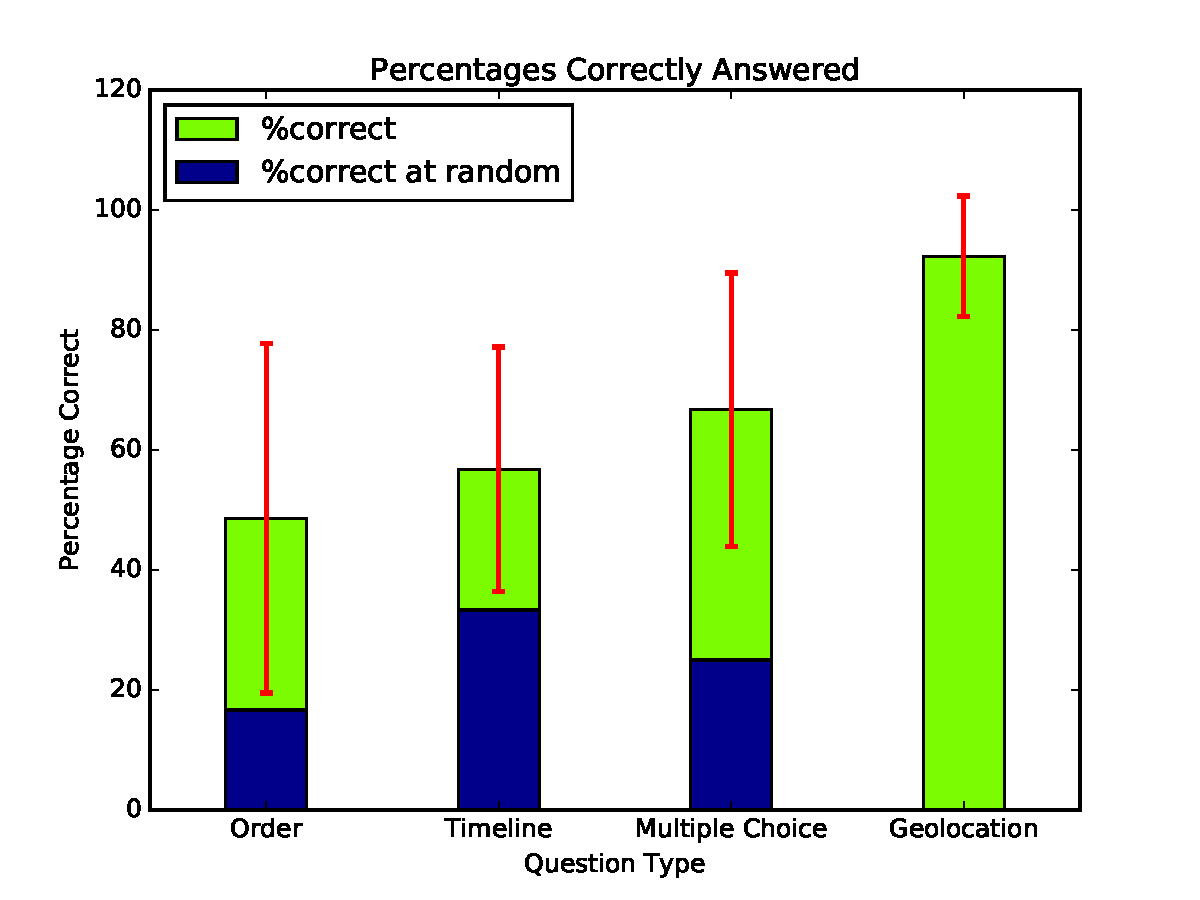
\includegraphics[width=4in]{images/pilot_2_correct.pdf}}
\caption{Percentages Correctly Answered}
\label{fig:p2Correct}
\end{figure}
\begin{figure}
\centering
{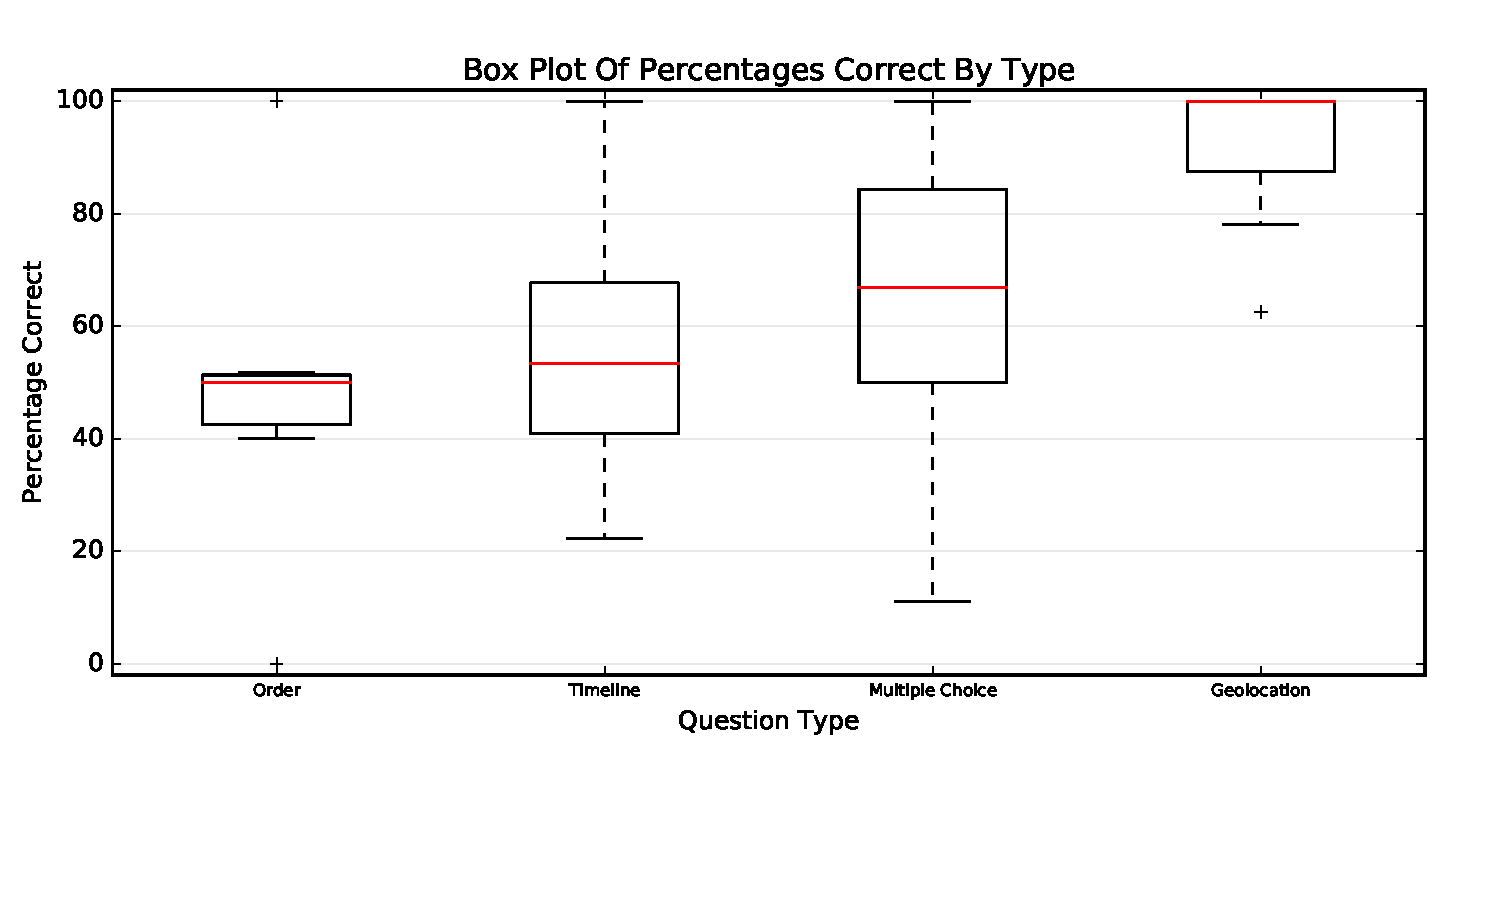
\includegraphics[width=4in]{images/pilot_2_boxplot.pdf}}
\caption{Percentages Correctly Answered Box Plots}
\label{fig:p2Boxes}
\end{figure}

\subsection{The results in more details}
\subsubsection{Ordering Questions}
The ordering questions results suggest that our question generating algorithm may be making slightly too harsh questions. The algorithm was designed to bring a user closer to a 50\% success rate over time, so the more a user play the closer they should get to 50\%. Figure \ref{fig:ordScatter} shows a scatter plot of the success rate of the players relative to their number of games played. The scatter plot shows no particular tendency.

\begin{figure}
\centering
{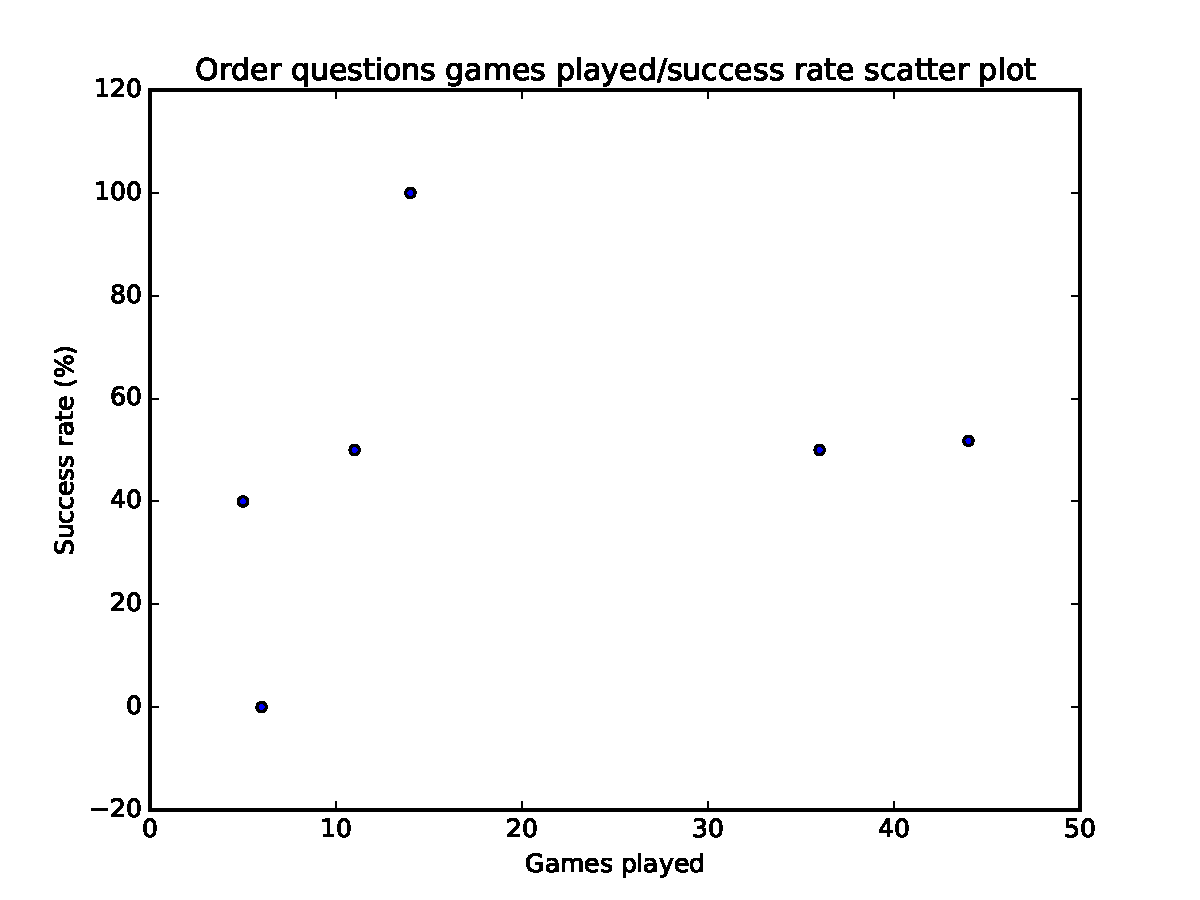
\includegraphics[width=4in]{images/order_scatter.pdf}}
\caption{Order questions games played/success rate scatter plot}
\label{fig:ordScatter}
\end{figure}

\subsubsection{Timeline Questions}
The box plot from section \ref{sec:p2remem} seems to suggest that the questions may be too easy but the range is quite large. The scatter plot on figure \ref{fig:timeScatter} shows that there is no clear patter as to how the number of games played impact the success rate.
\begin{figure}
\centering
{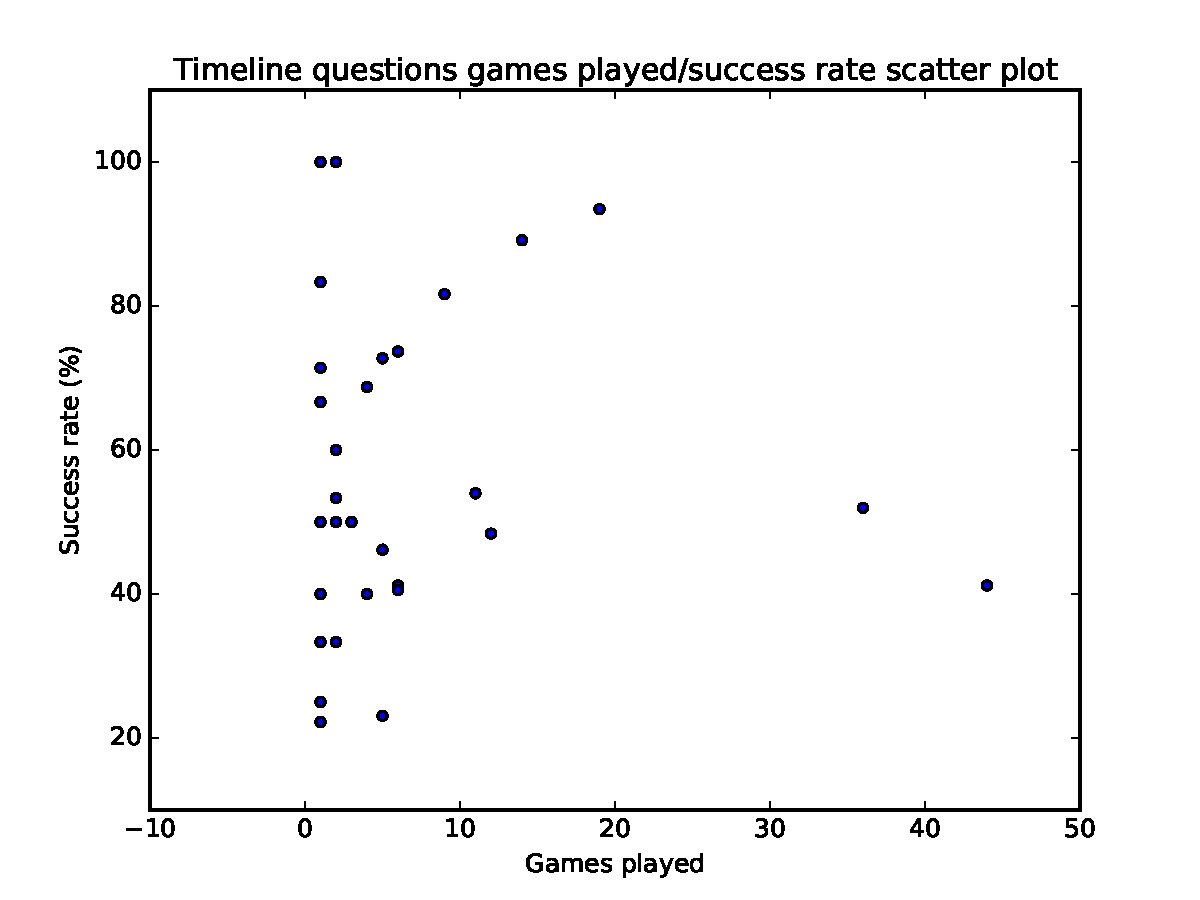
\includegraphics[width=4in]{images/timeline_scatter.pdf}}
\caption{Timeline questions games played/success rate scatter plot}
\label{fig:timeScatter}
\end{figure}

\subsubsection{Multiple Choice}
The box plot from section \ref{sec:p2remem} suggests that the questions are too easy. The scatter plot on figure \ref{fig:mcScatter} shows that there is no clear patter as to how the number of games played impact the success rate.
\begin{figure}
\centering
{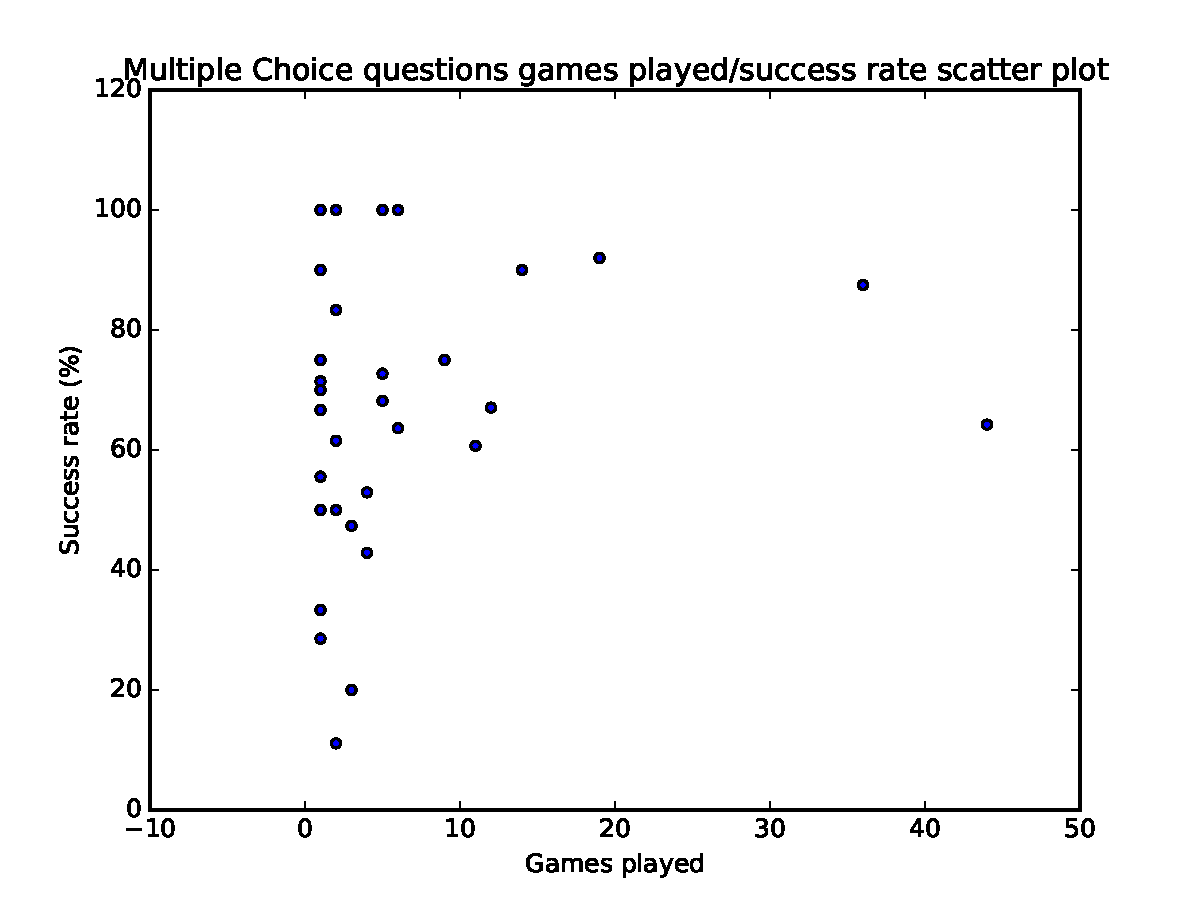
\includegraphics[width=4in]{images/mc_scatter.pdf}}
\caption{Multiple Choice questions games played/success rate scatter plot}
\label{fig:mcScatter}
\end{figure}
\subsubsection{Geolocation}\label{subsec:geolocissue}
Let's first start with the scatter plot of figure \ref{fig:geoScatter}. It exhibits the same shape as the other scatter plots, only that nearly all the players have a success rate of more than 75\%. Which implies that the impact of the amount of games played on the success rate follows no particular pattern.

\begin{figure}
\centering
{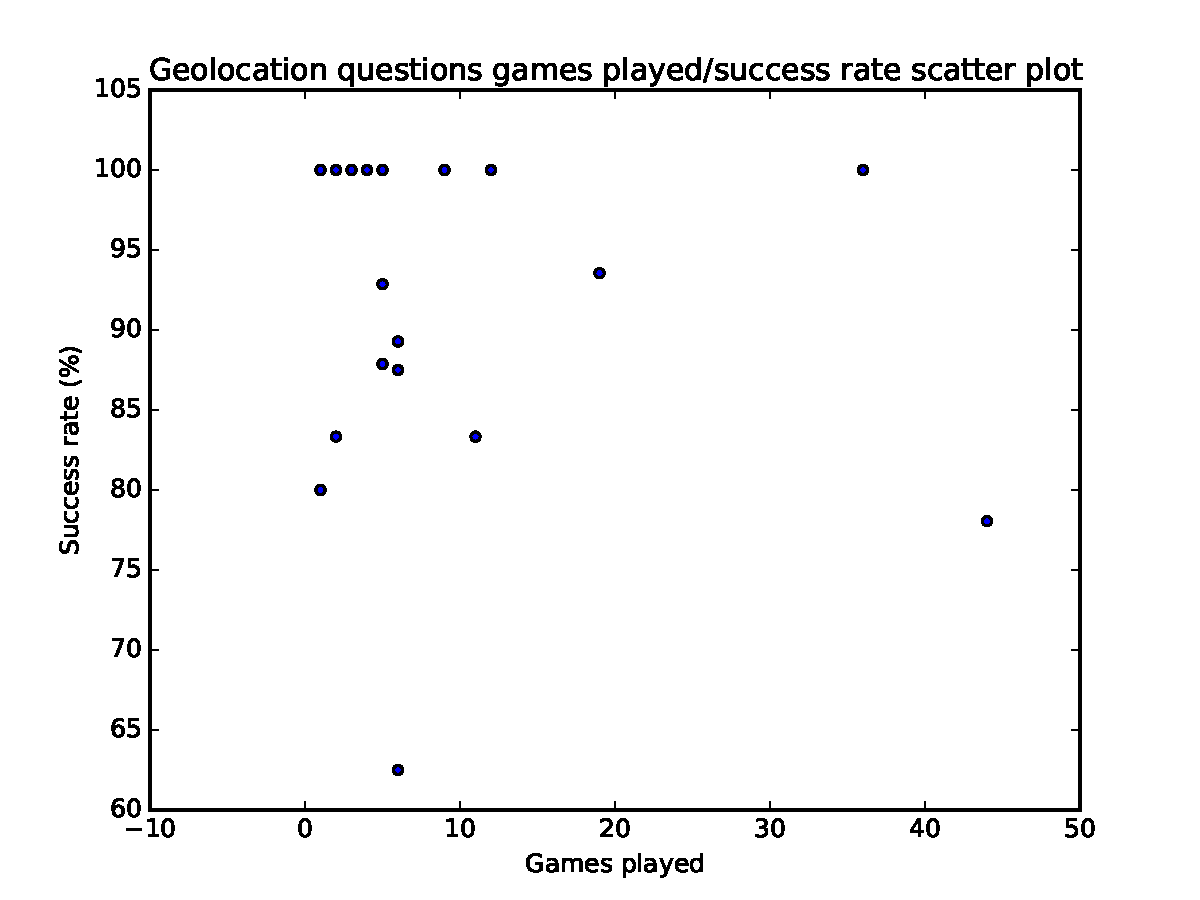
\includegraphics[width=4in]{images/geo_scatter.pdf}}
\caption{Geolocation questions games played/success rate scatter plot}
\label{fig:geoScatter}
\end{figure}

\subsection{Results explanation}\label{subsec:explained}
First we need to ask ourselves how different the result of the second pilot are from the ones from the first one. Given the size of the data samples and their nature we decided to use some two sample T-tests to compare the performance results from the first and second pilot. The results of those tests are shown in table \ref{table:pvals}. With such P-values it is impossible to tell whether or not the changes had an impact on the performance of the users.\\\\
The first possible reason for this result is the choice of the parameters we chose to adapt the difficulty. It is possible that we did not take into account some useful parameters and used some less useful ones. To investigate this possibility we would need to run other tests with other sets of parameters.\\\\
Another reason can be the heuristic used to generate a board. There was a strong focus to find questions of a certain difficulty. Doing so narrows down a lot the amount of possible items and might lead to asking the same question a lot of times. In fact this probably played a huge role in the results we observed for the Geolocation questions. Among the 613 generated Geolocation questions, we observed only 145 unique questions and one of them even appeared as much as 83 times. On average the players were then presented with the same Geolocation question 4.23 times. This results in those questions being really easy to answer. We expect the same to be true for other kind of question but we did not have time to confirm that yet.

\begin{table}[ht]
\caption{Two sample T-tests results}
\centering
\begin{tabular}{c c}
\hline\hline
Question Type & P-value \\ [0.5ex]

\hline
Order & 0.28143059003724213 \\
Timeline & 0.29291393698682511 \\
Multiple Choice & 0.45063940703557148 \\
Geolocation & 0.72398403288466295 \\ [1ex]
\hline
\end{tabular}
\label{table:pvals}
\end{table}

\subsection{What about the time spent?}
As suggested by figure \ref{fig:p2BoxesTime}, the timing results are pretty much the same as in the first pilot.
\begin{figure}
\centering
{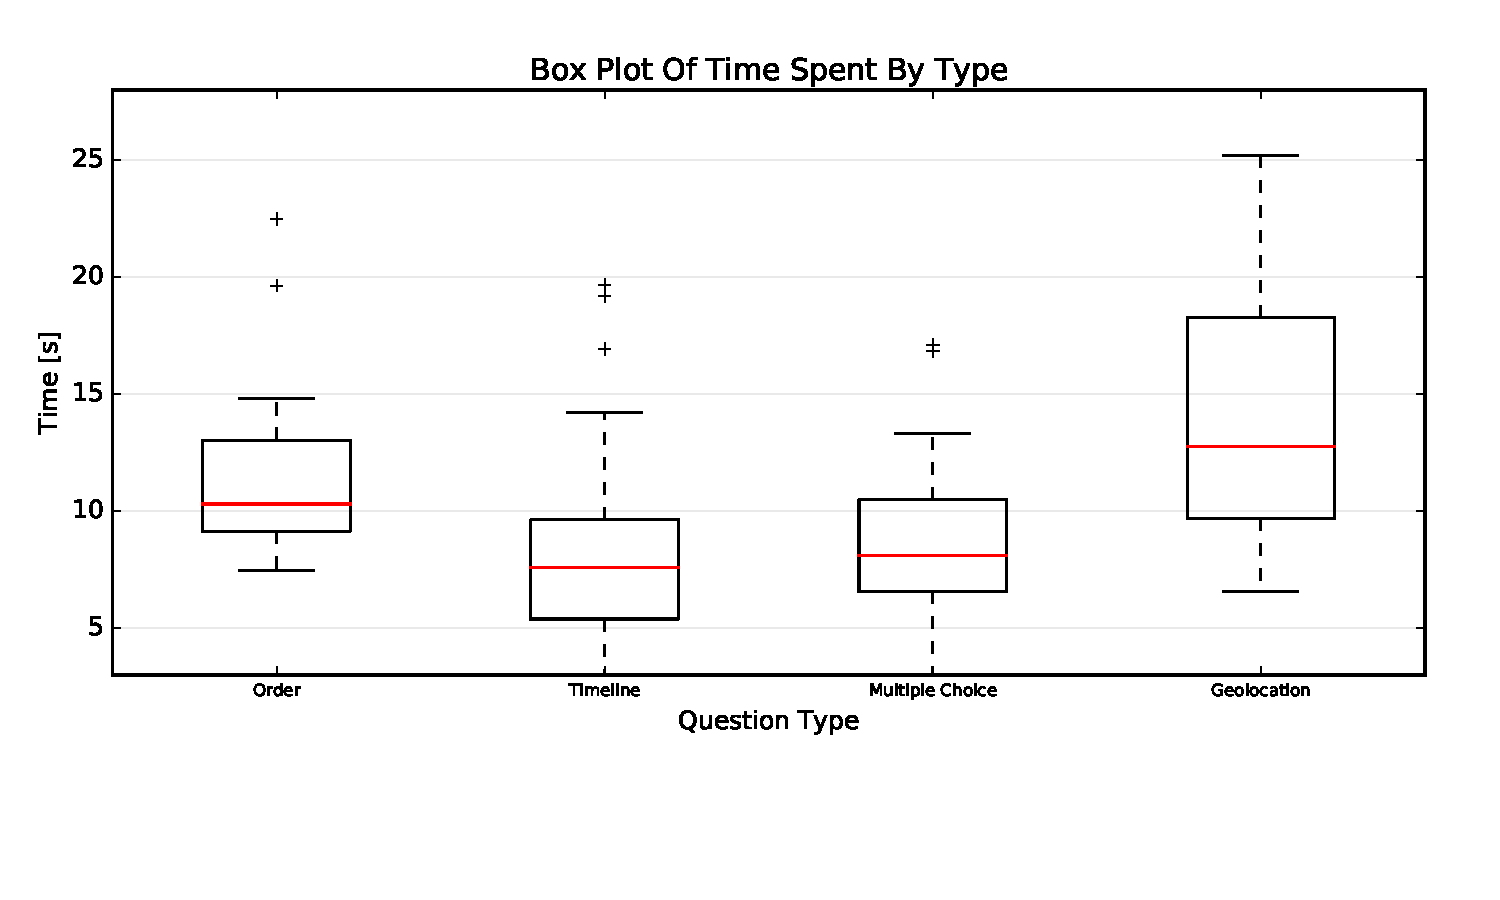
\includegraphics[width=4in]{images/pilot_2_boxplot_time.pdf}}
\caption{Box Plots Of Time Spent By Type}
\label{fig:p2BoxesTime}
\end{figure}

\subsection{Some general feedback}
There is also some feedback not directly linked to question difficulty that we got and are worth discussing. First of all, people enjoyed playing the game and they had a good time answering questions. This is really important for us as providing entertainment is key to having a lot of users participating in the surveys.\\\\
Then, in some cases, the participant reported that they got a question about a post which content was really uninteresting and therefore hard to identify. For instance, we had someone who had a post with only "Done" as text. We already use some basic techniques to avoid having empty posts, but some more advanced techniques might need to be used (such as machine learning and natural language processing\cite{nlp}) to avoid such cases if we deem it necessary.\\\\
Finally, on a somewhat related issue, it was reported that the questions about posts containing only a link are inconvenient to answer as one would need to click on the link in order to identify the shared article or video most of the time. We can address this issue by using the Facebook Graph API which allows us to request more information about a post's attachments which could give us the extra information we need to generate better link questions.